
  %judul bisa diketik ulang
  \setstretch{1}%\small
  \begin{center}
      \textbf{\large \Title}\\
      \bigskip 
  \end{center}
  
  
  
  %Nama authors
  \begin{center}
    \bf \Author$^1$, Mira Kania Sabariah$^2$, Monterico Adrian$^3$
  \end{center}
  
  
  %Afiliasi dan email
  \begin{center}
    $^{1,2,3}$Fakultas Informatika, Universitas Telkom, Bandung\\
$^1$rovino@students.telkomuniversity.ac.id, $^2$mirakarnia@telkomuniversity.ac.id,\\ $^3$monterico@telkomuniversity.ac.id
  \end{center}
  
  
%%% Abstrak Indonesia %%%%%%%%%%  
  \newpage
{\bf \parindent0pt \noindent\rule{\textwidth}{1pt}}
Abstrak

Meningkatnya jumlah pelanggan yang mengantri untuk mendapatkan layanan di bank, restoran, rumah sakit, dan tempat lainnya di Indonesia menyebabkan antrian yang panjang, yang berdampak pada kenyamanan dan kepuasan pelanggan serta mutu layanan. Saat ini, sistem antrian manual masih banyak digunakan, di mana pelanggan harus menunggu di tempat hingga giliran mereka tiba. Sistem ini kurang efisien dan tidak fleksibel bagi pelanggan yang ingin menghemat waktu. Oleh karena itu, diperlukan solusi antrian yang lebih modern dan efektif. Penggunaan aplikasi antrian berbasis web menjadi solusi penting untuk mengatasi masalah ini, dengan memungkinkan pelanggan mengantri secara virtual dari jarak jauh. Penelitian ini mengusulkan pengembangan aplikasi antrian menggunakan arsitektur monolitik dengan \textit{NestJs} dan \textit{PrismaJs} sebagai \textit{framework} utamanya. Arsitektur ini dipilih karena kemudahan pengembangan dan penerapannya pada tahap awal, serta fleksibilitasnya untuk migrasi ke arsitektur \textit{microservice} jika diperlukan di masa depan. \textit{NestJs} mendukung pengembangan aplikasi yang \textit{scalable} dan terstruktur, sementara \textit{PrismaJs} sebagai ORM memudahkan manajemen \textit{database} yang kompleks. Aplikasi ini juga mengimplementasikan otentikasi \textit{JWT} untuk keamanan dan menerapkan prinsip desain yang baik untuk menghindari \textit{anti-pattern}. Hasil pengujian menunjukkan bahwa aplikasi ini memiliki kualitas kode yang baik dengan \textit{code coverage} yang tinggi sebesar 96,32\% pada \textit{unit testing} dan performa yang memadai dalam \textit{stress testing}, meskipun masih ada area yang perlu dioptimalkan, seperti efisiensi fungsi tertentu. Kontribusi utama dari penelitian ini adalah pengembangan sistem antrian yang lebih efektif dan efisien dengan arsitektur yang dapat berkembang sesuai kebutuhan, serta penerapan praktik pengembangan perangkat lunak yang memperhatikan aspek keamanan, dan \textit{maintainability}.

\bigskip
Kata kunci : NestJS, PrismaJS, Anti-Pattern, Antrian, Backend, REST
\newpage



%%% Abstrak English %%%%%%%%%%  


\newpage

\noindent\rule{\textwidth}{1pt}
Abstract

The increasing number of customers queuing for services at banks, restaurants, hospitals, and other places in Indonesia leads to long queues, which affects customer comfort, satisfaction, and service quality. Currently, manual queuing systems are still widely used, where customers have to wait on-site until their turn arrives. This system is inefficient and inflexible for customers who want to save time. Therefore, a more modern and effective queuing solution is needed. The use of web-based queuing applications becomes an essential solution to address this problem by allowing customers to queue virtually from a distance. This research proposes the development of a queuing application using a monolithic architecture with \textit{NestJs} and \textit{PrismaJs} as the main frameworks. This architecture is chosen for its ease of development and deployment in the initial stages, as well as its flexibility to migrate to a \textit{microservice} architecture if needed in the future. \textit{NestJs} supports the development of scalable and well-structured applications, while \textit{PrismaJs} as an ORM facilitates the management of complex databases. The application also implements \textit{JWT} authentication for security and follows good design principles to avoid anti-patterns.
The test results indicate that the application has good code quality with a high code coverage of 96.32\% in unit testing and adequate performance in stress testing, although there are still areas that need optimization, such as the efficiency of certain functions. The main contribution of this research is the development of a more effective and efficient queuing system with an architecture that can evolve according to needs, along with the implementation of software development practices that consider aspects of security and maintainability.

\bigskip
Keywords: NestJS, PrismaJS, Anti-Pattern, Queue, Backend, REST

\noindent\rule{\textwidth}{1pt}
\newpage


%%%%%% isi paper %%%%

\section{Pendahuluan}

\noindent\textbf{Latar Belakang}

Meningkatnya populasi di indonesia mengakibatkan banyak pelanggan yang mengantri untuk mendapatkan layanan di bank, restoran, rumah sakit, dan tempat penyedia jasa lainnya. Mengantri merupakan kegiatan yang membosankan dan menguras waktu. Panjangnya antrian juga mampu berdampak pada mutu pelayanan di suatu tempat. Pelanggan yang harus menunggu lama berpotensi beralih ke pesaing, atau jika ada urusan lain yang lebih penting, maka pelanggan akan keluar dari tempat antrian, meninggalkan antriannya \cite{khong2017queue}\cite{Ghazal2016}\cite{Uddin2016}. Solusi yang ada pada bank, kantor pos, dan rumah sakit saat ini menggunakan \textit{ticketting} nomor antrian secara manual, di mana antrian yang sedang dilayani ditampilkan di layar pada ruang tunggu. Hal ini kurang efektif karena pelanggan harus berada di ruang tunggu\cite{Ghazal2016}.

Perkembangan teknologi yang cepat mengakibatkan penggunaan perangkat pintar atau \textit{smartphone} merupakan hal lumrah, banyak bermunculan aplikasi antrian virtual seperti Antrique, Qiwee, ExaQue di mana pengguna dapat mengantri dari jarak jauh melalui aplikasi maupun \textit{website}. Para pengguna aplikasi tersebut dapat melakukan hal lain saat mengantri sebelum gilirannya. Namun, aplikasi-aplikasi tersebut memiliki kelemahan seperti tidak ada estimasi waktu antrian, dan masih belum ada yang berfokus ke sektor \textit{food and beverage}.

Oleh karena itu, perlunya dikembangkan sebuah aplikasi yang memiliki \textit{feature} yang sama atau lebih dengan menutup kekurangan pada aplikasi tersebut. Pengembangan aplikasi menggunakan arsitektur monolitik karena mudahnya untuk dibuat dan di-\textit{deploy} secara cepat untuk iterasi awal. Arsitektur monolitik memungkinkan proses pengembangan dan deployment lebih efisien dalam skala kecil. Namun, arsitektur monolitik memiliki kelemahan seperti sulitnya untuk di-\textit{maintenance}, \textit{scale}, dan \textit{reliability} nya. Oleh karena itu, perlu dipertimbangkan kemungkinan migrasi ke arsitektur \textit{microservice} seiring dengan berkembangnya kebutuhan dan cakupan aplikasi \cite{gos2020comparison} \cite{jatkiewicz2023differences}.

Dalam pengembangan aplikasi \textit{web}, pemilihan bahasa pemrograman untuk digunakan di \textit{backend} sangatlah penting karena dapat memengaruhi performa aplikasi yang dibangun. Dalam pemilihan bahasa pemrograman \textit{backend}, banyak pilihan yang tersedia seperti PHP, Python, Ruby, PERL, dan banyak lagi. NodeJs merupakan \textit{tools} yang memungkinkan bahasa JavaScript dapat dijalankan pada sisi \textit{backend}. Dalam sisi performa, NodeJs lebih unggul dibanding PHP dan Python dalam sisi kecepatan melayani \textit{request} dari \textit{client} \cite{William2020} \cite{Odeniran2023}.

NestJs adalah \textit{framework backend} untuk Node.js yang menggunakan TypeScript dan dapat digunakan untuk pengembangan arsitektur \textit{microservice} maupun monolitik. Hal ini memungkinkan migrasi yang mudah dari arsitektur monolitik ke \textit{microservice} jika diperlukan. NestJs dapat digabungkan secara efektif dengan \textit{framework} PrismaJs untuk mengelola \textit{database} \cite{NestJS}. PrismaJs adalah \textit{framework Object Relational Mapping} (ORM) \cite{Prisma}, yang dirancang untuk mempercepat dan mempermudah pengembangan aplikasi dengan relasi \textit{database} yang kompleks dan sulit di-maintain menggunakan pendekatan \textit{Structured Query Language} (SQL) tradisional \cite{Zmaranda2020}. PrismaJs menawarkan keunggulan signifikan, termasuk keamanan tipe data yang kuat dengan TypeScript, migrasi \textit{database} yang mudah, performa yang lebih tinggi dibanding TypeOrm \cite{jamil2024use} \cite{kahvic2024prestandajamforelse}, dan pengalaman query yang disederhanakan. Kombinasi ini memungkinkan pengembang untuk membangun aplikasi yang \textit{scalable} dan \textit{maintainable}, serta mempermudah migrasi dari arsitektur monolitik ke arsitektur \textit{microservice} di masa depan.


Implementasi \textit{Application Programming Interface} (API) yang digunakan adalah \textit{Representational State Transfer} (RESTful) API, RESTful API adalah arsitektur untuk mempermudah komunikasi \textit{client-server} agar efektif untuk transaksi data. Namun, pada implementasi RESTful API, ada beberapa hal yang perlu diperhatikan seperti keamanan saat transaksi  atau komunikasi \cite{Beer2018}. Keamanan yang lemah dapat mengakibatkan \textit{hacker} dapat dengan mudah melakukan \textit{request tampering}, mengambil data pengguna, dan dapat membocorkan data keuangan mitra. Selain itu, penggunaan pola desain (\textit{design pattern}) yang tepat sangat penting untuk menghindari terjadinya \textit{anti-pattern}, yaitu praktik yang tidak dianjurkan atau kesalahan umum yang sering terjadi dalam pengembangan API. Menghindari \textit{anti-pattern} seperti penamaan endpoint yang tidak konsisten, \textit{over-fetching}, dan \textit{under-fetching} dapat meningkatkan kemampuan aplikasi untuk di-maintain dan di-sustain dalam jangka panjang \cite{Aghajani2018} \cite{Alshraiedeh2021}.

Berdasarkan uraian di atas, penelitian ini akan membuat sebuah \textit{backend} aplikasi antrian dengan menggunakan arsitektur monolitik dengan \textit{framework} NestJs dan PrismaJs sebagai \textit{framework} nya. Setelah \textit{features} aplikasi dibuat, perlu dilakukan unit testing untuk memvalidasi \textit{code} yang telah ditulis. Hal ini bertujuan untuk meminimalkan \textit{bug} dan mencegah terjadinya regresi saat \textit{feature} baru ditambahkan \cite{runeson2006survey}.

\noindent\textbf{Topik dan Batasannya}

Aplikasi Antria memerlukan \textit{backend} developer untuk mengimplementasikan fungsi fungsi API dan manajemen \textit{database} nya. Maka dapat dirumuskan permasalahan sebagai berikut:
\begin{enumerate}
  \item Bagaimana mengembangkan \textit{software} dengan \textit{index} \textit{maintainability} tinggi.
  \item Bagaimana merancang API yang bebas dari \textit{anti pattern}.
  \item Bagaimana merancang sistem keamanan pada API untuk melayani \textit{request}.
\end{enumerate}
dan batasan masalah sebagai berikut:
\begin{enumerate}
  \item Hanya berfokus kepada implementasi \textit{database} menggunakan Prisma ORM.
  \item \textit{Berfokus} ke bagaimana membuat \textit{endpoint} API yang tidak menimbulkan \textit{anti pattern}.
  \item Implementasi keamanan pada saat penanganan \textit{request} menggunakan \textit{JSON Web Token} (JWT).
\end{enumerate}


\noindent\textbf{Tujuan}

Tujuan dari pengerjaan Tugas Akhir ini yaitu:
\begin{enumerate}
  \item Mengimplementasikan Prisma ORM untuk mencapai \textit{index} \textit{maintainability} tinggi pada proyek.
  \item Membuat API yang dapat dengan mudah dimengerti dan di \textit{maintain}.
  \item Mengamankan data pengguna dengan memerlukan \textit{Authorization} pada setiap \textit{request header}.
  
\end{enumerate}

% \noindent \textbf{Organisasi Tulisan}

% Pada sub-bagian ini dituliskan bagian-bagian selanjutnya (setelah Pendahuluan) pada jurnal TA ini, disertai penjelasan sangat singkat.
\newpage

\section{Kajian Pustaka}
\subsection{NodeJs}
NodeJs adalah \textit{runtime} javascript yang basisnya dibangun dari V8 Java-Script \textit{Engine}. NodeJs berjalan dalam bentuk \textit{event-driven}, dan menggunakan model \textit{non blocking I/O}. meskipun menggunakan \textit{event-driven} untuk melayani \textit{request}, NodeJs dapat melayani jutaan koneksi dalam waktu bersamaan secara \textit{asynchronous} \cite{shah2017node}.

\subsection{NestJs}
NestJs merupakan \textit{framework} untuk Nodejs yang dikembangkan oleh Kamil Myśliwiec yang bertujuan untuk membuat aplikasi NodeJs yang efektif dan \textit{scalable}. NestJs mendukung penggunaan bahasa typescript dan javascript. NestJs juga menggabungkan komponen-komponen dari \textit{Functional Programming, Object Oriented Programming}, dan \textit{Functional Reactive Programming} \cite{pham2020developing} \cite{NestJS}.

\subsection{Object Relational Mapping}
\textit{Object Relational Mapping} (ORM) adalah sebuah teknologi yang memetakan tabel \textit{database} ke dalam objek, biasanya dipakai dalam bahasa yang berbasis \textit{Object Oriented Programming}. Dengan menggunakan ORM, developer dapat berfokus ke \textit{business logic} tanpa mengkhawatirkan penggunaan akses \textit{database} yang rumit \cite{lorenz2017object}. 

\subsection{PrismaJs}
PrismaJs adalah ORM \textit{Open} \textit{Source}, biasanya digunakan sebagai alternatif dari menggunakan \textit{Structured Query Language} (SQL) secara langsung. PrismaJs mendukung penggunaan \textit{database} MySQL, PostgreSQL, SQLite, SQL Server, CockroachDB, dan MongoDB. PrismaJs digunakan untuk mempermudah pengembangan \textit{database} yang memiliki relasi yang kompleks dan besar, dengan cara memberikan API yang \textit{type-safe} untuk \textit{query} \textit{database} nya dan mengembalikan hasil \textit{query} dalam bentuk \textit{JavaScript Object Notation} (JSON) \cite{Prisma}.

\subsection{Arsitektur Monolitik}
Arsitektur Monolitik adalah arsitektur sebuah \textit{software} dimana beberapa fungsi komponen yang berbeda seperti fungsi otorisasi, \textit{business logic}, notifikasi, dan pembayaran. Semua fungsi tersebut berada dalam satu program dan \textit{platform} yang sama. Arsitektur monolitik mudah untuk dikembangkan dan di-\textit{deploy}. Namun, sulit untuk di-\textit{maintenance} dan di-\textit{scale} \cite{gos2020comparison}. 


\subsection{JSON Web Token}
\textit{JSON Web Token} (JWT) adalah sebuah \textit{token} berbentuk \textit{string} json yang dapat digunakan untuk melakukan otorisasi. Ukuran JWT tergolong kecil jadi dapat dengan cepat di transfer antar \textit{client} dan \textit{server}. JWT menggunakan algoritma HMAC atau RSA untuk mengenkripsi \textit{digital signature} yang digunakan. JWT memiliki 3 bagian pada \textit{string} nya yang dipisahkan menggunakan ".", bagian ini berupa \textit{header}, \textit{payload}, dan \textit{signature} \cite{rahmatullo2019stateless}.

\subsection{Anti Pattern}
\textit{Anti Pattern} terjadi jika pembuatan nama sebuah objek tidak konsisten dengan yang lain. Objek di sini dapat berupa \textit{endpoint} API, nama \textit{variable}, nama fungsi, dan nama lain yang penggunaan nya bersifat publik. Terjadinya \textit{anti pattern} dapat mengakibatkan sulitnya untuk memahami suatu dokumentasi dan \textit{code} aplikasi \cite{Aghajani2018} \cite{Alshraiedeh2021}.

\subsection{RESTful API}
\textit{Representational State Transfer} (RESTful) \textit{Application Programming Interface} (API) adalah arsitektur untuk mempermudah komunikasi \textit{client-server} agar efektif untuk transaksi data. Tipe data yang paling sering digunakan untuk transaksi \textit{client} \textit{server} adalah JSON. Karakteristik RESTful meliputi : \textit{Client-Server}, \textit{Stateless}, \textit{Layered Architecture}, \textit{Caching}, \textit{Code on Demand}, dan \textit{Uniform Interface} \cite{giessler2015best}.

\newpage
\section{Sistem yang Dibangun}

Implementasi dan perancangan RESTful API, \textit{Database}, dan fungsi bisnis dikembangkan menggunakan \textit{framework} NestJs. Pada NestJs terdapat beberapa komponen seperti: \textit{Middleware}, \textit{Guards}, \textit{Interceptor}, \textit{Controller}, dan \textit{Service}. \textit{Service} yang dipakai adalah PrismaJs untuk menghubungkan NestJs ke \textit{Database System}. Desain arsitektur sistem secara keseluruhan pada gambar \ref{sistem-desain-arsitektur}. Terdapat 3 Aplikasi \textit{frontend} yang saling terhubung via \textit{backend}, Aplikasi Pelanggan berupa flutter, Aplikasi Mitra berupa flutter, dan \textit{Website} \textit{Dashboard} Mitra berupa ReactJs.
\begin{figure}[h]
  \centering
  \includegraphics[width=0.73\textwidth]{drawio/System-Design-Architecture.drawio.pdf}
  \caption{Arsitektur Desain Sistem}
  \label{sistem-desain-arsitektur}
\end{figure}
\newpage
\subsection{Request Life Cycle}
Gambar \ref{sistem-desain} merupakan \textit{Request Lifecycle} yang menjelaskan manajemen API atau bagaimana alur \textit{request} ditangani dari awal sampai akhir.
\begin{figure}[h]
  \centering
  \includegraphics[width=0.35\textwidth]{drawio/sistem-desain.drawio.pdf}
  \caption{Desain Sistem}
  \label{sistem-desain}
\end{figure}
\subsubsection{Middleware}
Pada \textit{Middleware}, fungsi akan dipanggil sebelum masuk ke \textit{routing}. fungsi \textit{middleware} dapat mengakses data \textit{request} dan \textit{response}. beberapa fungsi \textit{Middleware} seperti \textit{logger}, dan cek notifikasi. Contoh penggunaan nya bisa dilihat pada \textit{listing} \ref{lst:middleware}, \textit{request} dapat di hentikan maupun di alihkan ke \textit{middleware} selanjutnya.
\begin{lstlisting}[caption={Middleware},label={lst:middleware}]
  export class LoggerMiddleware implements NestMiddleware {
    use(req: Request, res: Response, next: NextFunction) {
      console.log('Request...');
      next();
    }
  }  
\end{lstlisting}

\subsubsection{Guard}
Pada \textit{Guard}, \textit{request} akan dicek \textit{authenticity}, untuk mengetahui \textit{validitas} dari \textit{request} tersebut. Tahap ini juga akan dicek keamanan \textit{session} menggunakan JWT dan CSRF. Contoh penggunaan \textit{guard} seperti pada \textit{listing} \ref{lst:guard}, \textit{request} yang menuju suatu \textit{controller} akan di cek oleh \textit{guards}, jika memiliki otorisasi maka akan dilanjutkan ke \textit{controller}, jika tidak akan di \textit{reject} dengan \textit{response} \textit{forbidden} \textit{access}.
\begin{lstlisting}[caption={Penggunaan Guards pada Controller},label={lst:guard}]
  @UseGuards(AuthGuard)
  @Get('profile')
  getProfile(@Request() req) {
      return req.user;
  }
\end{lstlisting}


\subsubsection{Interceptor}
Setelah melalui \textit{Guard}, \textit{Request} akan masuk ke \textit{Interceptor}. Di mana jika suatu \textit{request} mempunyai suatu karakteristik yang ditentukan, maka akan menjalankan fungsi tambahan. \textit{Interceptor} terjadi ketika \textit{request} datang \textit{(pre)}, dan \textit{response} \textit{(post)}. Contoh implementasi \textit{Interceptor} terdapat pada \textit{listing} \ref{lst:interceptor}.
\begin{lstlisting}[caption={Interceptor},label={lst:interceptor}]
  @UseInterceptors(FileInterceptor('profile_picture',fileInterceptor()))
  async update(@Param('id') id: string, @Body() data: Karyawan, @UploadedFile() file: Express.Multer.File): Promise<Karyawan> {}
\end{lstlisting}

\subsubsection{Controller}
Setelah melewati \textit{Interceptor}, fungsi di \textit{Controller} akan dijalankan. Jika pada \textit{Controller} tersebut perlu data dari \textit{database} maka akan turun ke \textit{service} PrismaJs. Contoh karyawan \textit{controller} pada \textit{listing} \ref{lst:controller} di mana \textit{request} akan diteruskan ke \textit{service} setelah \textit{password} di \textit{hash}.
\begin{lstlisting}[caption={Controller},label={lst:controller}]
  @Controller('karyawan')
  @Post()
  async create(@Body() data: any): Promise<Karyawan> {
    const hashedPassword = await bcrypt.hash(data.password, 10);
    const karyawanData = { ...data, password: hashedPassword };
    return this.karyawanService.createKaryawan(karyawanData);
  }
\end{lstlisting}

\subsubsection{Service}
Pada \textit{Service}, fungsi akan melakukan \textit{database} \textit{call} menggunakan ORM ke \textit{database} MySQL yang akan di kembalikan (return) ke \textit{Controller}\cite{NestJS}. Contoh implementasi \textit{service} pada \textit{listing} \ref{lst:service} di mana berfungsi untuk mengambil banyak karyawan.
\begin{lstlisting}[caption={Service},label={lst:service}]
  async karyawans(params: {
    skip?: number;
    take?: number;
    cursor?: Prisma.KaryawanWhereUniqueInput;
    where?: Prisma.KaryawanWhereInput;
    orderBy?: Prisma.KaryawanOrderByWithRelationInput;
  }): Promise<Karyawan[]> {
    const { skip, take, cursor, where, orderBy } = params;
    return this.prisma.karyawan.findMany({
      skip,take,cursor,where,orderBy,
    });
  }
\end{lstlisting}

\subsection{Persiapan}
Untuk memulai proyek, ada beberapa tahap yang perlu dilakukan, pertama membuat proyek nestjs menggunakan node, lalu dilanjutkan meng-\textit{install} dependensi yang diperlukan

\subsubsection{Instalasi NestJS dan Prisma}
Hal pertama yang dilakukan untuk meng-\textit{install} NestJS adalah membuka terminal lalu menjalankan \textit{command} npm untuk menginstall NestJS, di lanjut dengan meng-\textit{install} prisma \textit{client}.
\begin{lstlisting}[caption={terminal: npm},label={lst:npm_install}]
  $ npm i -g @nestjs/cli
  $ nest new antria
  $ npm install prisma --save-dev
\end{lstlisting}
\textit{Command} pada \textit{listing} \ref{lst:npm_install} untuk melakukan generasi \textit{folder} proyek pada NestJS, dan meng-\textit{install} prisma \textit{client} sebagai dependensi. Prisma sendiri merupakan aplikasi CLI untuk membantu dalam manajemen \textit{database} pada proyek NestJS menggunakan ORM.

\subsubsection{Konfigurasi Prisma}
Berdasarkan SRS, didapatkan beberapa \textit{entity} pada \textit{database} meliputi: Pelanggan, Mitra, Produk, OrderList, Pesanan, Antrian, Karyawan, Review, dan Analytic. Implementasi juga harus sesuai dengan \textit{Entity Relationship Diagram} (ERD) yang telah dibuat pada gambar \ref{erd}.
\begin{lstlisting}[caption={terminal: npx},label={lst:npx_prisma}]
  $ npx prisma init
  $ npx prisma migrate dev --name init
\end{lstlisting}
\textit{Command} pada \textit{listing} \ref{lst:npx_prisma} untuk inisialisasi prisma pada proyek, berfungsi untuk generasi\textit{ config template} yang nanti harus diubah, seperti \textit{database} \textit{connection} dan namA \textit{database} nya.
Pada tahap ini juga penulis perlu mendefinisikan model dan relasi pada \textit{database} ke bentuk notasi model prisma.
\begin{lstlisting}[caption={scheme.prisma},label={lst:scheme}]
  model Pesanan {
    invoice     String        @id
    payment     Payment
    pemesanan   OrderType?    @default(ONLINE)
    takeaway    Boolean       @default(false)
    status      PaymentStatus @default(PENDING)
    oderlist    OrderList[]
    pelanggan   Pelanggan     @relation(fields: [pelangganId], references: [id])
    pelangganId Int
    mitra       Mitra         @relation(fields: [mitraId], references: [id])
    mitraId     Int
    antrian     Antrian?
    antrianId   Int?
    created_at  DateTime      @default(now())
    updated_at  DateTime      @updatedAt
  }
  model OrderList {
    id        Int     @default(autoincrement()) @id
    quantity  Int     @default(1)
    note      String  @default("")
    pesanan   Pesanan @relation(fields: [pesananId], references: [invoice])
    produk    Produk  @relation(fields: [produkId], references: [id])
    produkId  Int
    pesananId String
  }
\end{lstlisting}
Pada \textit{listing} \ref{lst:scheme} penulis mendefinisikan skema model pesanan dan model orderlist beserta relasi nya pada prisma. \textit{syntax} \textit{@relation} berguna untuk mendefinisikan relasi nya pada model.

\begin{figure}[p]
  \centering
  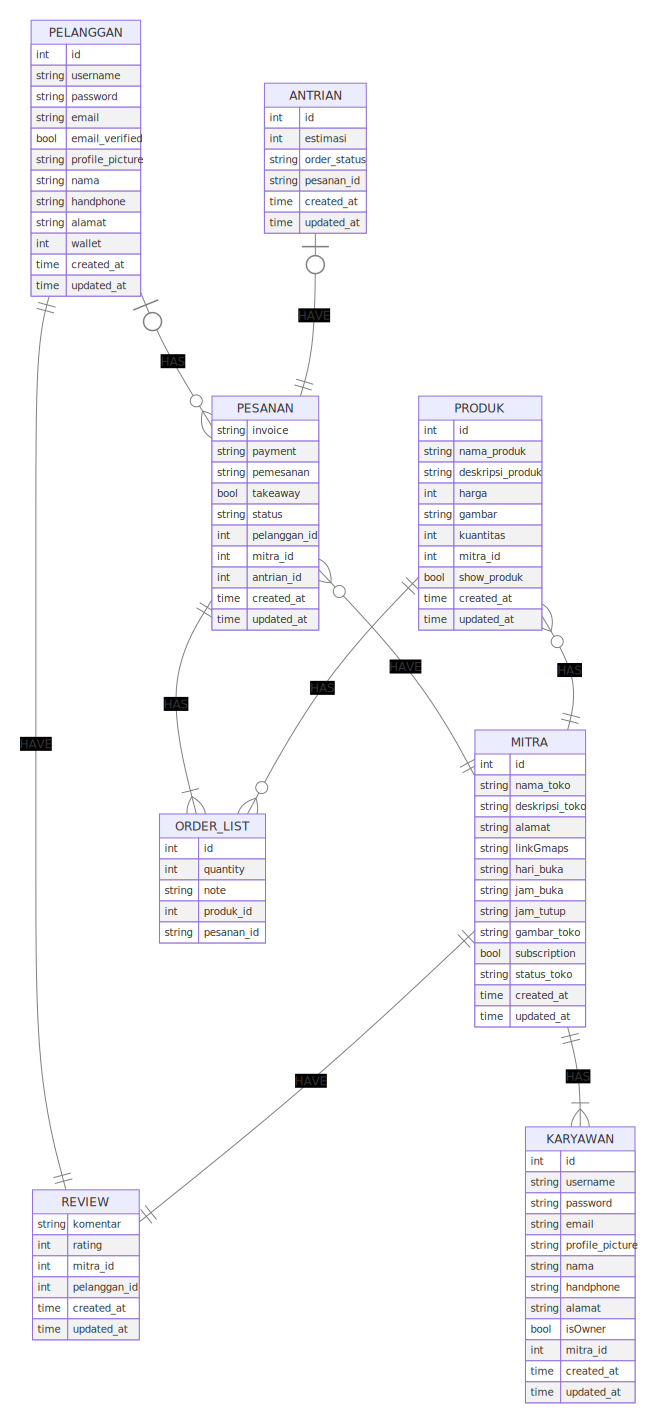
\includegraphics[width=1\textwidth]{drawio/erd.mermaid.png}
  \caption{Entity Relationship Diagram}
  \label{erd}
\end{figure}

\subsection{Implementasi}
\subsubsection{Guards}
implementasi \textit{code} \textit{guards} dibuat 2 fungsi, \textit{guards} untuk pengguna, dan \textit{guards} untuk mitra. Contoh implementasi pada \textit{listing} \ref{lst:authguards}, di sini penulis mendefinisikan \textit{guard} untuk memeriksa JWT \textit{Token} dari \textit{request} yang diterima apakah valid.
\begin{lstlisting}[caption={Authentication Guards}, label={lst:authguards}]
  export class AuthGuard implements CanActivate {
    constructor(private jwtService: JwtService) {}
    async canActivate(context: ExecutionContext): Promise<boolean> {
      const request = context.switchToHttp().getRequest();
      const token = this.extractTokenFromHeader(request);
      if (!token) {
        throw new UnauthorizedException();
      }
      try {
        const payload = await this.jwtService.verifyAsync(
          token,
          {
            secret: jwtConstants.secret
          }
        );
        request['user'] = payload;
      } catch {
        throw new UnauthorizedException();
      }
      return true;
    }
  
    private extractTokenFromHeader(request: Request): string | undefined {
      const [type, token] = request.headers.authorization?.split(' ') ?? [];
      return type === 'Bearer' ? token : undefined;
    }
  }
\end{lstlisting}

\subsubsection{Interceptor}
Contoh implementasi terdapat pada \textit{listing} \ref{lst:fileinterceptor}, di mana penulis mengimplementasikan \textit{interceptor} untuk mendeteksi dan mengambil \textit{file} dari \textit{multipart} \textit{request} data untuk diolah dan disimpan pada \textit{server}.
\begin{lstlisting}[caption={File Interceptor},label={lst:fileinterceptor}]
  @UseInterceptors(FileInterceptor('profile_picture',{
    storage: diskStorage({
      destination: "./MediaUpload/",
      filename: (req, file, callback) => {
        const uniqueSuffix = uuidv4();
        const fileExtName = path.extname(file.originalname);
        const newFileName = `${uniqueSuffix}${fileExtName}`;
        callback(null, newFileName);
      }
    })
  }))
\end{lstlisting}

\subsubsection{Controller}
\textit{Controller} minimal mengikuti banyak \textit{entity} pada model. masing masing \textit{controller} memiliki 4 fungsi yang merepresentasikan \textit{method} http yaitu GET, POST, PUT, DELETE. Khusus untuk \textit{endpoint} DELETE, pada beberapa \textit{cotroller} data tidak secara langsung di hapus, namun hanya diubah status nya dari \textit{enabled} ke \textit{disabled}.
\begin{enumerate}
  \item Pelanggan controller
  \item Mitra controller
  \item Produk controller
  \item OrderList controller
  \item Pesanan controller
  \item Antrian controller
  \item Karyawan controller
  \item Review controller
  \item Analytic controller
\end{enumerate}

\subsubsection{Service}
Sama seperti \textit{controller}, banyak \textit{service} minimal mengikuti banyak \textit{entity} pada model.
bedanya \textit{service} berinteraksi langsung dengan ORM Prisma.
\begin{enumerate}
  \item Pelanggan Service
  \item Mitra Service
  \item Produk Service
  \item OrderList Service
  \item Pesanan Service
  \item Antrian Service
  \item Karyawan Service
  \item Review Service
  \item Analytic Service
\end{enumerate}

\subsubsection{API Endpoint}
Untuk menghindari Anti Pattern, API \textit{endpoint} sesuai dengan nama \textit{entity} pada model.
setiap \textit{endpoint} entity mendukung 4 \textit{method} http yaitu POST, GET, PUT, dan DELETE.
\begin{enumerate}
  \item Auth Endpoint,
  Tabel \ref{tbl:auth} memetakan \textit{controller} auth pada \textit{endpoint} REST API.
  \begin{longtable}{| p{3.5cm} | p{1.5cm} | p{8cm} |}
    \caption{Auth Endpoint Table} \label{tbl:auth} \\
    \hline
    \textbf{Path} & \textbf{Method} & \textbf{Description} \\
    \hline
    \endfirsthead
    
    \multicolumn{3}{c}%
    {{\bfseries \tablename\ \thetable{} -- continued from previous page}} \\
    \hline
    \textbf{Path} & \textbf{Method} & \textbf{Description} \\
    \hline
    \endhead
    
    \hline \multicolumn{3}{|r|}{{Continued on next page}} \\ \hline
    \endfoot
    
    \hline
    \endlastfoot
    
    /auth/login/pelanggan & POST  & Endpoint untuk aplikasi mobile pelanggan, pengguna memasukkan credential login lalu akan mendapatkan JWT Token untuk mengakses enpoint API lain nya \\
    \hline
    /auth/login/mitra & POST & Endpoint untuk aplikasi mobile mitra, dan Web Dashboard. pengguna memasukkan credential login lalu akan mendapatkan JWT Token untuk mengakses enpoint API lain nya \\
    \hline
    
  \end{longtable}

  \item Pelanggan Endpoint,
  Tabel \ref{tbl:pelanggan} memetakan controller pelanggan pada endpoint REST API.
  \begin{longtable}{| p{2.5cm} | p{1.5cm} | p{9cm} |}
    \caption{Pelanggan Endpoint Table} \label{tbl:pelanggan} \\
    \hline
    \textbf{Path} & \textbf{Method} & \textbf{Description} \\
    \hline
    \endfirsthead
    
    \multicolumn{3}{c}%
    {{\bfseries \tablename\ \thetable{} -- continued from previous page}} \\
    \hline
    \textbf{Path} & \textbf{Method} & \textbf{Description} \\
    \hline
    \endhead
    
    \hline \multicolumn{3}{|r|}{{Continued on next page}} \\ \hline
    \endfoot
    
    \hline
    \endlastfoot
    
    /pelanggan & GET  & Endpoint untuk mengambil seluruh pelanggan terdaftar pada aplikasi \\
    \hline
    /pelanggan & POST  & Endpoint untuk membuat akun pelanggan baru \\
    \hline
    /pelanggan/\{id\} & GET  & Endpoint untuk mengambil akun pelanggan dengan id tertentu \\
    \hline
    /pelanggan/\{id\} & PUT  & Endpoint untuk memperbarui akun pelanggan dengan id tertentu \\
    \hline
    /pelanggan/\{id\} & DELETE  & Endpoint untuk menghapus (disable) akun pelanggan dengan id tertentu \\
    \hline
    
  \end{longtable}
  \item Karyawan Endpoint,
  Tabel \ref{tbl:karyawan} memetakan controller karyawan pada endpoint REST API.
  \begin{longtable}{| p{4.5cm} | p{1.5cm} | p{7cm} |}
    \caption{Karyawan Endpoint Table} \label{tbl:karyawan} \\
    \hline
    \textbf{Path} & \textbf{Method} & \textbf{Description} \\
    \hline
    \endfirsthead
    
    \multicolumn{3}{c}%
    {{\bfseries \tablename\ \thetable{} -- continued from previous page}} \\
    \hline
    \textbf{Path} & \textbf{Method} & \textbf{Description} \\
    \hline
    \endhead
    
    \hline \multicolumn{3}{|r|}{{Continued on next page}} \\ \hline
    \endfoot
    
    \hline
    \endlastfoot
    
    /karyawan & GET  & Endpoint untuk mengambil seluruh karyawan terdaftar pada aplikasi \\
    \hline
    /karyawan & POST  & Endpoint untuk membuat akun karyawan baru \\
    \hline
    /karyawan/\{id\} & GET  & Endpoint untuk mengambil akun karyawan dengan id tertentu \\
    \hline
    /karyawan/\{id\} & PUT  & Endpoint untuk memperbarui akun karyawan dengan id tertentu \\
    \hline
    /karyawan/\{id\} & DELETE  & Endpoint untuk disable akun karyawan dengan id tertentu \\
    \hline
    /karyawan/mitra/\{mitraId\} & GET  & Endpoint untuk mengambil seluruh karyawan terdaftar pada aplikasi dan id mitra tertentu \\
    \hline
    
  \end{longtable}

  \item Mitra Endpoint,
  Tabel \ref{tbl:mitra} memetakan controller mitra pada endpoint REST API.
  \begin{longtable}{| p{2cm} | p{1.5cm} | p{9.5cm} |}
    \caption{Mitra Endpoint Table} \label{tbl:mitra} \\
    \hline
    \textbf{Path} & \textbf{Method} & \textbf{Description} \\
    \hline
    \endfirsthead
    
    \multicolumn{3}{c}%
    {{\bfseries \tablename\ \thetable{} -- continued from previous page}} \\
    \hline
    \textbf{Path} & \textbf{Method} & \textbf{Description} \\
    \hline
    \endhead
    
    \hline \multicolumn{3}{|r|}{{Continued on next page}} \\ \hline
    \endfoot
    
    \hline
    \endlastfoot
    
    /mitra & GET  & Endpoint untuk mengambil seluruh mitra terdaftar pada aplikasi \\
    \hline
    /mitra & POST  & Endpoint untuk membuat akun mitra baru \\
    \hline
    /mitra/\{id\} & GET  & Endpoint untuk mengambil mitra dengan id tertentu \\
    \hline
    /mitra/\{id\} & PUT  & Endpoint untuk mengaupdate mitra dengan id tertentu \\
    \hline
    /mitra/\{id\} & DELETE  & Endpoint untuk menghapus (disable) mitra dengan id tertentu \\
    \hline
    
  \end{longtable}

  \item Produk Endpoint,
  Tabel \ref{tbl:produk} memetakan controller prduk pada endpoint REST API.
  \begin{longtable}{| p{3.5cm} | p{1.5cm} | p{8cm} |}
    \caption{Produk Endpoint Table} \label{tbl:produk} \\
    \hline
    \textbf{Path} & \textbf{Method} & \textbf{Description} \\
    \hline
    \endfirsthead
    
    \multicolumn{3}{c}%
    {{\bfseries \tablename\ \thetable{} -- continued from previous page}} \\
    \hline
    \textbf{Path} & \textbf{Method} & \textbf{Description} \\
    \hline
    \endhead
    
    \hline \multicolumn{3}{|r|}{{Continued on next page}} \\ \hline
    \endfoot
    
    \hline
    \endlastfoot
    
    /produk & GET  & Endpoint untuk mengambil seluruh produk yang terdaftar pada aplikasi \\
    \hline
    /produk & POST  & Endpoint untuk membuat produk baru pada mitra tertentu \\
    \hline
    /produk/\{id\} & GET  & Endpoint untuk mengambil prduk dengan id tertentu \\
    \hline
    /produk/\{id\} & PUT  & Endpoint untuk memperbarui produk dengan id tertentu \\
    \hline
    /produk/\{id\} & DELETE  & Endpoint untuk menghapus (disable) produk dengan id tertentu \\
    \hline
    /produk/mitra/\{mitraId\} & GET  & Endpoint untuk mengambil produk dari id mitra \\
    \hline
    
  \end{longtable}

  \item Pesanan Endpoint,
  Tabel \ref{tbl:pesanan} memetakan controller pesanan pada endpoint REST API.
  \begin{longtable}{| p{4cm} | p{1.5cm} | p{7.5cm} |}
    \caption{Pesanan Endpoint Table} \label{tbl:pesanan} \\
    \hline
    \textbf{Path} & \textbf{Method} & \textbf{Description} \\
    \hline
    \endfirsthead
    
    \multicolumn{3}{c}%
    {{\bfseries \tablename\ \thetable{} -- continued from previous page}} \\
    \hline
    \textbf{Path} & \textbf{Method} & \textbf{Description} \\
    \hline
    \endhead
    
    \hline \multicolumn{3}{|r|}{{Continued on next page}} \\ \hline
    \endfoot
    
    \hline
    \endlastfoot
    
    /pesanan & GET  & Endpoint untuk mengambil seluruh pesanan \\
    \hline
    /pesanan & POST  & Endpoint untuk membuat pesanan baru \\
    \hline
    /pesanan/\{invoice\} & GET  & Endpoint untuk mengambil pesanan dengan invoice tertentu \\
    \hline
    /pesanan/\{invoice\} & PUT  & Endpoint untuk memperbarui pesanan dengan invoice tertentu \\
    \hline
    /pesanan/\{invoice\} & DELETE  & Endpoint untuk menghapus (disable) pesanan dengan invoice tertentu \\
    \hline
    /pesanan/mitra/\{mitraId\} & GET  & Endpoint untuk mengambil seluruh pesanan dari id mitra tertentu \\
    \hline
    
  \end{longtable}

  \item OrderList Endpoint,
  Tabel \ref{tbl:orderlist} memetakan controller orderlist pada endpoint REST API.
  \begin{longtable}{| p{4cm} | p{1.5cm} | p{7.5cm} |}
    \caption{OrderList Endpoint Table} \label{tbl:orderlist} \\
    \hline
    \textbf{Path} & \textbf{Method} & \textbf{Description} \\
    \hline
    \endfirsthead
    
    \multicolumn{3}{c}%
    {{\bfseries \tablename\ \thetable{} -- continued from previous page}} \\
    \hline
    \textbf{Path} & \textbf{Method} & \textbf{Description} \\
    \hline
    \endhead
    
    \hline \multicolumn{3}{|r|}{{Continued on next page}} \\ \hline
    \endfoot
    
    \hline
    \endlastfoot
    
    /orderlist & POST  & Endpoint untuk membuat orderlist baru\\
    \hline
    /orderlist/\{id\} & GET  & Endpoint untuk mengambil orderlist dengan id tertentu\\
    \hline
    /orderlist/\{id\} & PUT  & Endpoint untuk memperbarui orderlist dengan id tertentu\\
    \hline
    /orderlist/\{id\} & DELETE  & Endpoint untuk menghapus (disable) orderlist dengan id tertentu\\
    \hline
    /orderlist/invoice/\{invoice\} & GET  & Endpoint untuk mengambil orderlist dengan invoice\\
    \hline
    
  \end{longtable}

  \item Antrian Endpoint,
  Tabel \ref{tbl:antrian} memetakan controller antrian pada endpoint REST API.
  \begin{longtable}{| p{4cm} | p{1.5cm} | p{7.5cm} |}
    \caption{Antrian Endpoint Table} \label{tbl:antrian} \\
    \hline
    \textbf{Path} & \textbf{Method} & \textbf{Description} \\
    \hline
    \endfirsthead
    
    \multicolumn{3}{c}%
    {{\bfseries \tablename\ \thetable{} -- continued from previous page}} \\
    \hline
    \textbf{Path} & \textbf{Method} & \textbf{Description} \\
    \hline
    \endhead
    
    \hline \multicolumn{3}{|r|}{{Continued on next page}} \\ \hline
    \endfoot
    
    \hline
    \endlastfoot
    
    /antrian & POST  & Endpoint untuk membuat antrian baru \\
    \hline
    /antrian/\{id\} & GET  & Endpoint untuk mengambil antrian dengan id tertentu \\
    \hline
    /antrian/\{id\} & PUT  & Endpoint untuk memperbarui antrian dengan id tertentu \\
    \hline
    /antrian/\{id\} & DELETE  &  Endpoint untuk menghapus (disable) antrian dengan id tertentu \\
    \hline
    /antrian/mitra/\{mitraId\} & GET  & Endpoint untuk mengambil antrian pada mitra tertentu \\
    \hline
    
  \end{longtable}

  \item Reviews Endpoint,
  Tabel \ref{tbl:review} memetakan controller review pada endpoint REST API.
  \begin{longtable}{| p{5cm} | p{1.5cm} | p{6.5cm} |}
    \caption{Reviews Endpoint Table} \label{tbl:review} \\
    \hline
    \textbf{Path} & \textbf{Method} & \textbf{Description} \\
    \hline
    \endfirsthead
    
    \multicolumn{3}{c}%
    {{\bfseries \tablename\ \thetable{} -- continued from previous page}} \\
    \hline
    \textbf{Path} & \textbf{Method} & \textbf{Description} \\
    \hline
    \endhead
    
    \hline \multicolumn{3}{|r|}{{Continued on next page}} \\ \hline
    \endfoot
    
    \hline
    \endlastfoot
    /reviews & GET  & Endpoint untuk mengambil seluruh review \\
    \hline
    /reviews & POST  & Endpoint untuk membuat review baru \\
    \hline
    /reviews/mitra/\{mitraId\} & GET  & Endpoint untuk mengambil review pada mitra tertentu \\
    \hline
    /reviews/\{mitraId\}/\{pelangganId\} & GET  & Endpoint untuk mengambil review pelanggan pada mitra\\
    \hline
    /reviews/\{mitraId\}/\{pelangganId\} & PUT  & Endpoint untuk memperbarui review pelanggan pada mitra \\
    \hline
    /reviews/\{mitraId\}/\{pelangganId\} & DELETE  & Endpoint untuk menghapus review pelanggan pada mitra\\
    \hline
    
  \end{longtable}

  \item Image server endpoint,
  endpoint pada tabel \ref{tbl:imageserver} untuk menyajikan gambar ke client melalui REST API.
  \begin{longtable}{| p{3cm} | p{1.5cm} | p{8.5cm} |}
    \caption{Image server Endpoint Table} \label{tbl:imageserver} \\
    \hline
    \textbf{Path} & \textbf{Method} & \textbf{Description} \\
    \hline
    \endfirsthead
    
    \multicolumn{3}{c}%
    {{\bfseries \tablename\ \thetable{} -- continued from previous page}} \\
    \hline
    \textbf{Path} & \textbf{Method} & \textbf{Description} \\
    \hline
    \endhead
    
    \hline \multicolumn{3}{|r|}{{Continued on next page}} \\ \hline
    \endfoot
    
    \hline
    \endlastfoot
    /image/\{fileName\} & GET  & Endpoint untuk menampilkan gambar dengan filename tertentu\\
    \hline
    
  \end{longtable}
\end{enumerate}

\subsection{Alur Pengujian}
Pengujian menggunakan metode \textit{white} \textit{box} testing yaitu unit testing. Testing dilakukan pada setiap fungsi yang telah dibuat tanpa terhubung ke komponen lain. Setelah semua fungsi lulus unit testing, dilakukan analisis statis menggunakan SonarQube untuk mengetahui indeks \textit{Maintainability}, \textit{Reliability}, dan \textit{Security}. Diagram alur pengujian dapat dilihat pada gambar \ref{alur-testing}.

\begin{figure}[h]
  {\centering {\includegraphics[scale=0.6]{drawio/alur-testing.png}}\par}
  \caption{Alur Testing}
  \label{alur-testing}
\end{figure}

\subsubsection{Unit Testing}
Pengujian dimulai dengan membuat \textit{file} yang bernama component.spec.ts seperti terlihat pada gambar \ref{ut1}. Lalu pada \textit{file} tersebut penulis mendeskripsikan \textit{test} apa yang akan dibuat seperti contoh pada \textit{listing} \ref{lst:jest-testing}, pertama definisikan parameter yang diperlukan \textit{function} lalu \textit{expect} hasil keluaran fungsi sesuai dengan yang ditentukan.
\begin{figure}[h]
  {\centering {\includegraphics[scale=1]{drawio/unit-testing1.png}}\par}
  \caption{File spec.ts}
  \label{ut1}
\end{figure}

\begin{lstlisting}[caption={Contoh Testing Menggunakan Jest},label={lst:jest-testing}]
  describe('canActivate', () => {
  it('should return true if user role is karyawan', async () => {
    const mockRequest = { user: { role: 'karyawan' } };
    const mockContext = { switchToHttp: () => ({ getRequest: () => mockRequest }) } as unknown as ExecutionContext;

    expect(await guard.canActivate(mockContext)).toBe(true);
  });

  it('should return false if user role is not karyawan', async () => {
    const mockRequest = { user: { role: 'admin' } };
    const mockContext = { switchToHttp: () => ({ getRequest: () => mockRequest }) } as unknown as ExecutionContext;

    expect(await guard.canActivate(mockContext)).toBe(false);
  });
});
\end{lstlisting}
\subsubsection{Maintainability Testing}
Pengujian terhadap aspek \textit{maintainability} dari perangkat lunak dilakukan dengan menggunakan alat analisis statis bernama \textit{SonarQube}. Alat ini memberikan penilaian berupa indeks \textit{rating} yang di kategori-kan dalam tingkatan A, B, C, D, dan E, yang masing-masing mencerminkan tingkat kualitas dari tiga aspek utama, yaitu \textit{Security} (keamanan), \textit{Reliability} (keandalan), dan \textit{maintainability} (kemudahan pemeliharaan). Tingkatan A menunjukkan kualitas terbaik, sedangkan E menunjukkan kualitas terendah. Dengan menggunakan \textit{SonarQube}, penulis dapat mengidentifikasi area dalam kode yang memerlukan perbaikan untuk meningkatkan kualitas perangkat lunak secara keseluruhan.

\newpage

\subsection{Deployment}
Ketika \textit{backend} selesai di kembangkan dan siap dipakai maka akan dilakukan \textit{deployment}.
Pada diagram \ref{deployment} menjelaskan bagaimana \textit{server} \textit{backend} berkomunikasi dengan Aplikasi lain melalui protokol HTTPS dan memiliki \textit{database} pusat yaitu di \textit{backend} untuk sinkronisasi data dari satu aplikasi ke aplikasi lain. 

\begin{figure}[h]
  {\centering {\includegraphics[scale=0.6]{drawio/deployment.jpg}}\par}
  \caption{Deployment Diagram}
  \label{deployment}
\end{figure}

\newpage

\section{Evaluasi}
\subsection{Endpoint Anti Pattern}
Untuk mengevaluasi pattern pada endpoint yang telah dibuat perlu adanya standarisasi penamaan endpoint berdasarkan \cite{cs7194} seperti berikut :
\begin{lstlisting}[caption={Format penamaan endpoint dasar},label={lst:endpoint1level}]
  untuk GET all dan POST sebuah entity
  /entity
  untuk GET id dan DELETE sebuah entity
  /entity/{entity_id}
\end{lstlisting}
Enpoint tersebut telah mencakup seluruh method yang diperlukan REST API, namun jika memerlukan data yang terhubung dengan entity lain maka didefinisikan format sebagai berikut :
\begin{lstlisting}[caption={Format penamaan endpoint entity from entity},label={lst:endpoint2level}]
  untuk GET seluruh entity Berdasarkan entity kedua
  /entity/2nd_entity/{2nd_entity_id}
  Untuk GET,UPDATE, dan DELETE Entity dengan composite Key antara 2 entity
  /entity/{2nd_entity_id}/{3rd_entity_id}
\end{lstlisting}
Lalu ada juga endpoint dimana entity pertama melakukan fungsi terhadap entity kedua dengan format :
\begin{lstlisting}[caption={Format penamaan endpoint entity function to entity},label={lst:endpointfunction}]
  /entity/function/2nd_entity
\end{lstlisting}
Dari format diatas dapat dievaluasi endpoint API yang telah dibuat :
\begin{longtable}{| p{10cm} | p{1.5cm} | p{1.5cm} |}
  \caption{Evaluasi Endpoint Anti Pattern} \label{tbl:anti-pattern} \\
  \hline
  \textbf{Path} & \textbf{Method} & \textbf{Evaluasi} \\
  \hline
  \endfirsthead
  \multicolumn{3}{c}%
  {{\bfseries \tablename\ \thetable{} -- continued from previous page}} \\
  \hline
  \textbf{Path} & \textbf{Method} & \textbf{Evaluasi} \\
  \hline
  \endhead
  \hline \multicolumn{3}{|r|}{{Continued on next page}} \\ \hline
  \endfoot
  \hline
  \endlastfoot
  /auth/login/pelanggan & POST  & SESUAI \\
  \hline
  /auth/login/mitra & POST & SESUAI \\
  \hline
  /pelanggan & GET  & SESUAI \\
  \hline
  /pelanggan & POST  & SESUAI \\
  \hline
  /pelanggan/\{id\} & GET  & SESUAI \\
  \hline
  /pelanggan/\{id\} & PUT  & SESUAI \\
  \hline
  /pelanggan/\{id\} & DELETE  & SESUAI \\
  \hline
  /karyawan & GET  & SESUAI \\
  \hline
  /karyawan & POST  & SESUAI \\
  \hline
  /karyawan/\{id\} & GET  & SESUAI \\
  \hline
  /karyawan/\{id\} & PUT  & SESUAI \\
  \hline
  /karyawan/\{id\} & DELETE  & SESUAI \\
  \hline
  /karyawan/mitra/\{mitraId\} & GET  & SESUAI \\
  \hline
  /mitra & GET  & SESUAI \\
  \hline
  /mitra & POST  & SESUAI \\
  \hline
  /mitra/\{id\} & GET  & SESUAI \\
  \hline
  /mitra/\{id\} & PUT  & SESUAI \\
  \hline
  /mitra/\{id\} & DELETE  & SESUAI \\
  \hline
  /produk & GET  & SESUAI \\
  \hline
  /produk & POST  & SESUAI \\
  \hline
  /produk/\{id\} & GET  & SESUAI \\
  \hline
  /produk/\{id\} & PUT  & SESUAI \\
  \hline
  /produk/\{id\} & DELETE  & SESUAI \\
  \hline
  /produk/mitra/\{mitraId\} & GET  & SESUAI \\
  \hline
  /pesanan & GET  & SESUAI \\
  \hline
  /pesanan & POST  & SESUAI \\
  \hline
  /pesanan/\{invoice\} & GET  & SESUAI \\
  \hline
  /pesanan/\{invoice\} & PUT  & SESUAI \\
  \hline
  /pesanan/\{invoice\} & DELETE  & SESUAI \\
  \hline
  /pesanan/mitra/\{mitraId\} & GET  & SESUAI \\
  \hline
  /orderlist & POST  & SESUAI \\
  \hline
  /orderlist/\{id\} & GET  & SESUAI \\
  \hline
  /orderlist/\{id\} & PUT  & SESUAI \\
  \hline
  /orderlist/\{id\} & DELETE  & SESUAI \\
  \hline
  /orderlist/invoice/\{invoice\} & GET  & SESUAI \\
  \hline
  /antrian & POST  & SESUAI \\
  \hline
  /antrian/\{id\} & GET  & SESUAI \\
  \hline
  /antrian/\{id\} & PUT  & SESUAI \\
  \hline
  /antrian/\{id\} & DELETE  &  SESUAI \\
  \hline
  /antrian/mitra/\{mitraId\} & GET  & SESUAI \\
  \hline
  /reviews & GET  & SESUAI \\
  \hline
  /reviews & POST  & SESUAI \\
  \hline
  /reviews/mitra/\{mitraId\} & GET  & SESUAI \\
  \hline
  /reviews/\{mitraId\}/\{pelangganId\} & GET  & SESUAI \\
  \hline
  /reviews/\{mitraId\}/\{pelangganId\} & PUT  & SESUAI \\
  \hline
  /reviews/\{mitraId\}/\{pelangganId\} & DELETE  & SESUAI \\
  \hline
  /image/\{fileName\} & GET  & SESUAI \\
  \hline

\end{longtable}



\subsection{Hasil Pengujian}
\subsubsection{Unit Testing}
Untuk unit testing, terdapat 2 \textit{Test} \textit{suite} pada setiap \textit{entity} kecuali auth di mana auth memiliki 3 \textit{test} \textit{suite} yang di total sebanyak 21 \textit{test} \textit{suite} yang perlu dibuat dan dilakukan.

\begin{figure}[h]
  {\centering {\includegraphics[scale=0.8]{drawio/unitTesting.png}}\par}
  \caption{Hasil unit testing menggunakan jest}
  \label{unit-testing}
\end{figure}

\begin{figure}[h]
  {\centering {\includegraphics[scale=0.9]{drawio/CoverageSummary.png}}\par}
  \caption{Coverage Summary}
  \label{coverage-summary}
\end{figure}

\newpage

\subsubsection{Maintainability Testing}
Pada bagian ini, penulis melakukan pengujian menggunakan \textit{SonarQube} dan \textit{Sonar Scanner} untuk menganalisis kode program yang telah dibuat. Proses analisis ini bertujuan untuk mengevaluasi kualitas kode dengan mengidentifikasi potensi masalah dalam aspek \textit{Security}, \textit{Reliability}, dan \textit{Maintainability}. Setelah analisis selesai, \textit{SonarQube} memberikan skor indeks yang mencerminkan tingkat kualitas kode dalam kategori-kategori tersebut. Skor ini membantu penulis memahami area mana yang perlu ditingkatkan untuk memastikan kode yang lebih aman, andal, dan mudah dipelihara.
\begin{figure}[H]
  {\centering {\includegraphics[scale=0.5]{drawio/maintainability-1.png}}\par}
  \caption{Hasil Analysis SonarQube}
  \label{maintainability-testing-1}
\end{figure}
\begin{figure}[H]
  {\centering {\includegraphics[scale=0.63]{drawio/maintainability-2.png}}\par}
  \caption{Cognitive Complexity Melebihi treshold untuk fungsi createPesanan}
  \label{maintainability-testing-2}
\end{figure}

\newpage

\subsection{Analisis Hasil Pengujian}
\subsubsection{Unit Testing}
Semua \textit{test case} pada unit testing lolos uji atau \textit{pass} dengan \textit{code coverage} 96,32\% dengan LOC (Line Of Code) sekitar 524 dari 544 LOC. Jika dilihat pada gambar \ref{unit-testing}, LOC yang tidak teruji terdapat pada \textit{file} karyawan, mitra, pelanggan, dan produk. Kode yang tidak teruji berupa \textit{interceptor} untuk mendeteksi \textit{file} gambar pada \textit{multipart} \textit{request}, fungsi tersebut tidak dapat diuji pada unit testing dikarenakan perlunya \textit{request} autentik \textit{multipart} dan tidak bisa di simulasi-kan secara efektif.

\subsubsection{Maintainability Testing}
Pada gambar \ref{maintainability-testing-1} menunjukkan hasil analisis dari SonarQube bahwa kualitas kode secara keseluruhan memenuhi standar yang ditetapkan. Namun, ada beberapa area yang perlu diperhatikan terkait \textit{maintainability}. Persentase \textit{Duplications} adalah 12.9\%, yang menunjukkan adanya duplikasi kode dalam 5.9k baris kode. Meskipun ini tidak secara langsung memengaruhi \textit{maintainability} dalam skala besar, pengurangan duplikasi dapat meningkatkan kualitas kode secara keseluruhan. Pada aspek \textit{maintainability}, SonarQube memberikan penilaian A, yang menunjukkan tingkat \textit{maintainability} yang baik. Namun, pada gambar \ref{maintainability-testing-2}, ada satu isu khusus yang perlu diperbaiki: fungsi \texttt{createPesanan}. Fungsi ini memiliki \textit{Cognitive Complexity} sebesar 16, yang melebihi batas yang diizinkan yaitu 15. Untuk meningkatkan \textit{maintainability}, disarankan untuk merestrukturisasi fungsi ini agar \textit{Cognitive Complexity} dapat dikurangi, sehingga mempermudah pemahaman dan pemeliharaan kode di masa depan.
\section{Kesimpulan}

Berdasarkan implementasi dan perancangan sistem menggunakan NestJs dan Prisma, dapat diambil beberapa kesimpulan terkait Anti Pattern, Keamanan, dan Maintainabilitas.
\begin{enumerate}
  \item \textbf{Anti Pattern}\newline
  Penting untuk menghindari Anti Pattern dalam pengembangan aplikasi, yaitu praktik yang tidak dianjurkan atau kesalahan umum yang sering dilakukan. Dalam sistem yang dikembangkan, beberapa langkah yang telah diambil untuk menghindari Anti Pattern meliputi:
  \begin{itemize}
    \item \textbf{Penamaan Endpoint yang konsisten}
    \item \textbf{Separation of Concerns}: Memisahkan setiap komponen dalam aplikasi (Middleware, Guards, Interceptor, Controller, dan Service) sesuai dengan tanggung jawab masing-masing.
    \item \textbf{Menghindari Over-fetching dan Under-fetching}
  \end{itemize}
  \item \textbf{keamanan}\newline
  Keamanan adalah aspek penting dalam pengembangan aplikasi, dan penelitian ini menunjukkan bahwa langkah-langkah yang diambil untuk memastikan keamanan sistem telah berhasil diterapkan dengan baik. Beberapa langkah yang diimplementasikan meliputi:

  \begin{itemize}
    \item \textbf{JWT Authentication}: Penggunaan JWT untuk otentikasi dan otorisasi pengguna, yang memastikan hanya pengguna yang valid dapat mengakses endpoint tertentu, sehingga meningkatkan keamanan akses aplikasi.
    \item \textbf{Data Validation}: Validasi data diterapkan pada setiap layer aplikasi (Controller, Service) untuk menjaga integritas dan keamanan data, mengurangi risiko serangan injeksi dan data yang tidak valid.
    \item \textbf{Encryption}: Penggunaan bcrypt untuk meng-hash password pengguna sebelum disimpan di database, melindungi data sensitif dari potensi kebocoran atau akses tidak sah.
  \end{itemize}
  Selain itu, analisis menggunakan SonarQube menunjukkan bahwa kualitas kode terkait keamanan memenuhi standar yang ditetapkan, dengan identifikasi dan mitigasi kerentanan yang efektif. SonarQube memberikan penilaian positif terhadap keamanan kode, namun juga menyoroti area-area yang masih perlu diperhatikan untuk meningkatkan keamanan lebih lanjut.

  \item \textbf{Maintainabilitas}\newline
  Hasil penelitian menunjukkan bahwa sistem yang dikembangkan menggunakan kombinasi \textit{NestJs} dan \textit{PrismaJs} memiliki tingkat maintainabilitas yang tinggi. \textit{NestJs} menerapkan prinsip \textit{Separation of Concerns} dengan memisahkan setiap komponen aplikasi seperti \textit{Controller}, \textit{Service}, \textit{Middleware}, \textit{Guards}, dan \textit{Interceptors} sesuai dengan tanggung jawab masing-masing, sehingga memudahkan pengembangan, pemeliharaan, dan pengujian komponen secara terpisah. Sementara itu, \textit{PrismaJs} sebagai ORM mempermudah manajemen \textit{database} yang kompleks dengan menyediakan struktur yang jelas, dukungan tipe data yang kuat, dan fitur migrasi yang intuitif. Kombinasi ini tidak hanya mempercepat pengembangan aplikasi, tetapi juga mempermudah proses pemeliharaan dan pengembangan lebih lanjut, menjadikannya solusi yang efektif untuk aplikasi yang memerlukan skalabilitas dan fleksibilitas tinggi.

\end{enumerate}
\newpage

\subsection{Saran}
Untuk meningkatkan performa dan skalabilitas sistem, terdapat beberapa hal yang perlu diperhatikan dan ditingkatkan, antara lain:
\begin{enumerate}
  \item \textbf{Performa} \newline
  \begin{itemize}
    \item \textbf{Tidak menggunakan Prisma ORM}: Penggunaan Prisma dapat meningkatkan maintainability dengan memangkas performa, dengan tidak menggunakan Prisma dan hanya menggunakan raw sql, dapat meningkatkan performa akses database.
  \end{itemize}
  \item \textbf{Skalabilitas} \newline
  \begin{itemize}
    \item \textbf{Microservices Architecture}: Pertimbangkan untuk memecah aplikasi menjadi beberapa layanan mikro yang independen. Hal ini dapat meningkatkan skalabilitas dan memudahkan pengembangan serta pemeliharaan setiap komponen.
    \item \textbf{Kubernetes and Containerization}: Gunakan teknologi container seperti Docker dan orkestrator container seperti Kubernetes untuk memudahkan pengelolaan dan skala aplikasi. Teknologi ini memungkinkan aplikasi dijalankan di berbagai lingkungan dengan konsistensi yang tinggi.
  \end{itemize}
\end{enumerate}
Dengan meningkatkan aspek-aspek ini, sistem diharapkan dapat beroperasi dengan lebih efisien dan mampu menangani pertumbuhan pengguna dan data di masa mendatang.

\newpage

\bibliographystyle{abbrv}
\bibliography{references}

\section*{Lampiran}
\noindent
Link Artefak: \url{https://drive.google.com/drive/folders/1fwESO-2QtJHrtzywm5PP2TCEnAkrmt4o?usp=sharing}
\newline
Link Aplikasi: \url{https://github.com/Soviena/antria-backend}